\chapter{系统设计}
\section{数据源选择}
我们所采用的数据\cite{Harper:2016bm}是由明尼苏达大学GroupLens研究小组提供的MovieLens数据。数据是真实的用户对于电影的评分,MovieLens数据从上世纪90年代开始收集,目前评分总数已经超过两千万条。我们采用的数据集数据主要划分五个部分。
\begin{itemize}
    \item 100k数据集。数据来源于1000用户对于1700部电影的评价,评分总数达到10万。使用5分制。
    \item 1M数据集。数据来源于6000用户对于4000部电影的评价,评分总数达到100万。使用5分制。
    \item 10M数据集。数据来源于72000用户对于10000部电影的评分。评分总数达到1000万。使用5分制,可以使用半分。
    \item 20M数据集。数据来源于138000用户对于27000部电影的评分。评分总数达到2000万。使用5分制,可以使用半分。
    \item small数据集。数据来源于668个用户对于10325部电影的评分,评分总数达到10万。使用5分制,可以使用半分。
\end{itemize}

\subsection{数据预处理部分}
标准提供的数据包含时间戳,并且几类数据采用不同的分割方式,由于我们不需要时间戳,并需要统一数据的表示。在预处理过程将时间戳去除,并统一每行数据的分割方式使用逗号进行分割。预处理过程我们可以在单机上完成,并不需要分布式。

\section{Spark架构搭建}
前面提及到,Spark框架由master节点和slave节点组成,在我们搭建的Spark集群中,使用了一台master节点和两台slave节点进行搭建。如下图\ref{fig:cluster}。
\begin{figure}[ht]
\centering
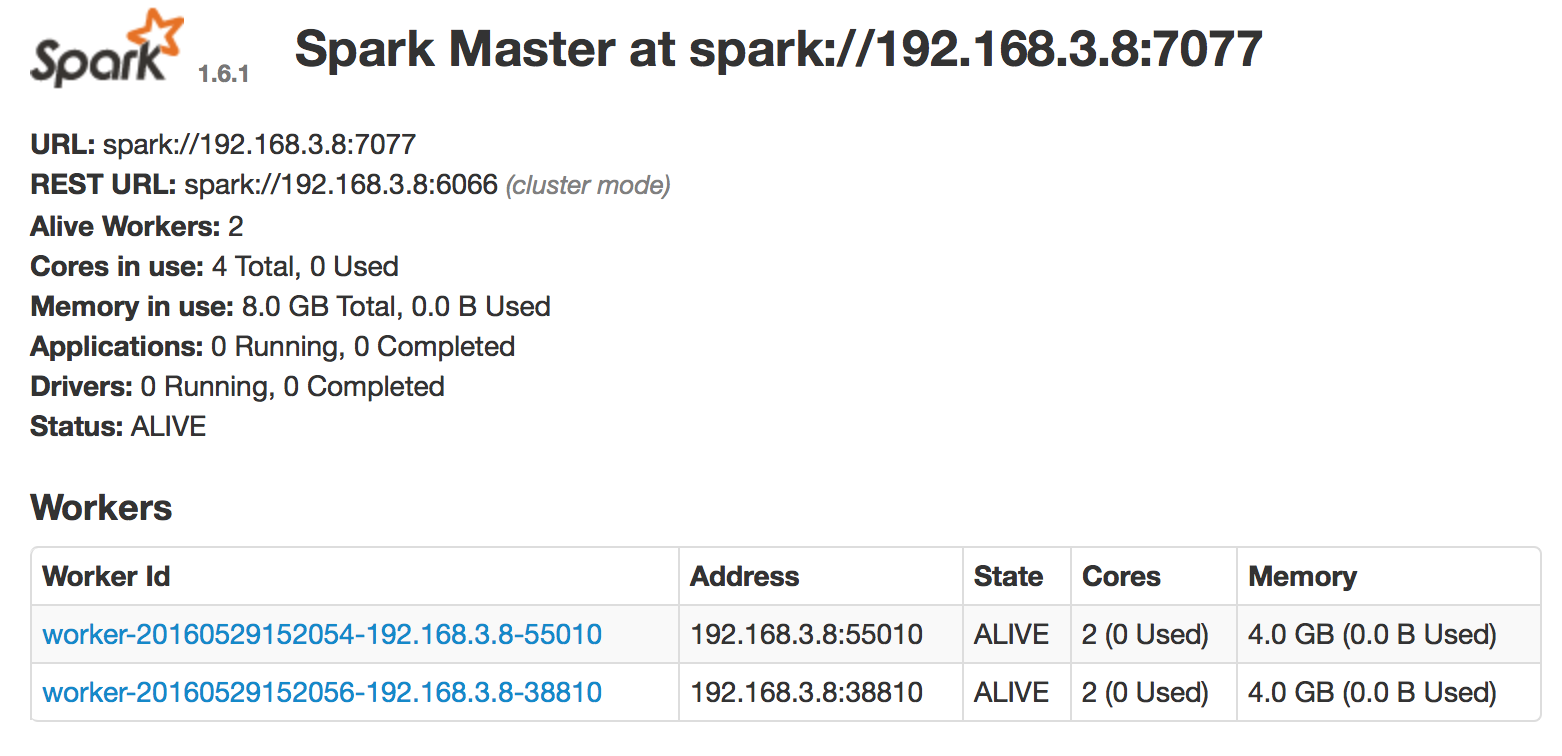
\includegraphics[width=15cm]{spark-cluster}
\caption{Spark cluster}\label{fig:cluster}
\end{figure}
Driver使用了2g内存,使用了两个work节点,每个work节点使用2个核,4G内存。

\section{并行算法设计}
前述描述基于邻域的推荐的算法时使用的是串行算法,无法进行并行化。下面我们设计并行化方法来实现基于邻域的推荐算法,而ALS算法由于本身迭代过程可以并行化,不需要做额外的修改。
    \begin{algorithm}
        \caption{相似性的并行计算}
        \begin{algorithmic}[1] %每行显示行号
            \Require \\
            \begin{itemize} 
                \item $M_{u, *}$, 一个代表用户-物品评分矩阵的的RDD,用户的索引作为键值。 每个$M_{u,*}$都代表一个评分或者为空。
                \item $Sim(((u, v), Seq(V)))$, 一个用户自定义的用来计算用户$u$和$v$余弦相似性的函数。 $V$是用户$u$和$v$都交互过的物品-物品评分评分对的列表。
                \item $SampleInteractions(K, Seq(V), n)$ 一个用户自定义的用来对$Seq(V)$进行采样的函数,如果$Seq(V)$的长度超过$n$,返回其本身,否则,就返回$Seq(V)$中的$n$个随机采样。
                \item $KeyOnFirstItem(((u, v), V)$, 是一个用户自定义的用来转换用来把 $(u, v)$转换成$u$并添加$v$到$V$值行程$(u, V)$对的函数。通常用来在单个物品上产生对。
                \item $NearestNeighbors(K, Seq(V), k)$是一个用户自定义的函数用来从邻居物品中选择最相似的K个物品。
                \item $Map(f, (K, V))$, $Filter(f, (K, V))$, and $GroupByKey((K, V))$ 像之前定义的一样,$(K, V)$ 代表一个RDD对象 ,$f$是一个用户自定义函数。
           \end{itemize}
            \Ensure $S_{u,v}$一个稀疏的用户相似性矩阵,每个 $S_{u, v}$ $\in [0, 1]$或者为空。

            \Function{PAIRWISEITEMS}{M, N}
            \State itemRatingPairs $\leftarrow$ Map(FindItemPairs(), Map(SampleInteractions(n), $M_{u, *}$))
            \State pairwiseItems $\leftarrow$ GroupByKey(itemRatingPairs)
            \State \textbf{emit} pairwiseItems
            \EndFunction
            \\
            \Function{ITEMSIMILARITY}{pairwiseItems, k}
                \State itemSims $\leftarrow$ Map(KeyOnFirstItem(), Map(Sim(), pairwiseItems)
                \State nearestItems $\leftarrow$ map(NearestNeighbors(k), GroupByKey(itemSims))
                \State \textbf{emit} nearestItems
            \EndFunction
        \end{algorithmic}
    \end{algorithm}
    
    \begin{algorithm}
    \caption{并行的Top-N推荐算法}
    \begin{algorithmic}[1]
        \Require \\
        \begin{itemize}
               \item $M_{u, *}$, 一个代表用户-物品评分矩阵的的RDD,用户的索引作为键值。 每个$M_{u,*}$都代表一个评分或者为空。
            \item $nearestItems$, 在$M$,中最相似的$K$个物品。这个变量需要用Spark broadcast方式初始化。
            \item $n$, 需要返回的n个推荐商品。
            \item $WeightedSums(K, V, NearestItems, n)$, 用户自定义的根据相似关系计算加权后的评分的函数。
            \item $Map(f, (K, V))$, $Filter(f, (K, V))$, and $GroupByKey((K, V))$ 像之前定义的一样,$(K, V)$ 代表一个RDD对象 ,$f$是一个用户自定义函数。
        \end{itemize}
        \Ensure itemRecs, 对一个用户评分最高的$n$个推荐商品
        \Function{GROUPITEMRATINGS}{M}
            \State UserItemRatings $\leftarrow$ GroupByKey($M_{u, *}$)
            \State \textbf{emit} UserItemRatings
        \EndFunction
        \\
        \Function{TOPNRECOMMENDATIONS}{UserItemRatings, NearestItems, n}
             \State ItemRecs $\leftarrow$ Map(WeightedSums(NearestItems, n), UserItemRatings)
            \State \textbf{emit} ItemRecs
        \EndFunction
    \end{algorithmic}
    \end{algorithm}

使用基于用户-用户的相似性计算和物品-物品的相似性计算所采用的算法主体框架基本相同,只需要在输入出稍微变化一下即可通用。在朴素的并行算法之外,我们在还对用户的评分总数进行了采样操作,通过采样,我们可以在保持运算精度的情况下降低运算时间,下一节在实验结果中我们会进行分析。

\subsection{算法复杂度分析}
我们先分析ALS算法中
$x_u = (Y W_u Y^T + \lambda I)^{-1} Y W_u q_u$这一步计算的复杂度。在求逆$Y W_u Y^T + \lambda I$中,我们忽略单位矩阵的影响,假设我们希望分解的特征数是$f$。所以$X = X_{m \times f}$和 $Y = Y_{f \times n}$。 对于$x_u$,求逆里面的运算复杂度是$O(f * n * f)$。 $f \times f$矩阵的求逆运算复杂度来说$O(f^3)$,之后乘法复杂度是$O(f*f*n)$和$O(f*n*1)$。所以对于求$x_u$的复杂度是$O(f^2n) + O(f^3) + O(f^2n) + O(fn) = O(n)$,求$y_i$的复杂度是$O(m)$。因为每次迭代,需要求$m$次$x_u$和$n$次$y_i$。得出单次迭代ALS算法的复杂度为$O(mn)$。

未加采样的的基于用户-用户的相似关系的推荐算法,最坏情况每个物品会产生$m^2$对用户评分组合,每个用户组合最多有$n$个共同交互的产品,复杂度是$O(m^2n)$,基于物品-物品的相似关系的推荐算法复杂度是$O(mn^2)$,通过加入sample采样数$K$,理论上将复杂度降低到了$O(K^2m)$或者$O(K^2n)$的复杂度,$K^2$是一个较大的常数。